\chapter{Running the Solver \texttt{xspecfem3D}}\label{cha:Running-the-Solver}

Now that you have successfully generated the databases, you are ready
to compile the solver. In the main directory, type
{\small
\begin{verbatim}
make xspecfem3D
\end{verbatim}
}
\noindent
Please note that \texttt{xspecfem3D} must be called directly from
the main directory, as most of the binaries of the package.\\

\noindent
The solver needs three input files in the \texttt{DATA} directory
to run:
\begin{description}
\item [{\texttt{Par\_file}}] the main parameter file which was discussed
in detail in the previous Chapter~\ref{cha:Creating-Distributed-Databases},
\item [{\texttt{CMTSOLUTION}} or {\texttt{FORCESOLUTION}}] the earthquake
source parameter file or the force source parameter file, and
\item [{\texttt{STATIONS}}] the stations file.
\end{description}
Most parameters in the \texttt{Par\_file} should be set prior to running
the databases generation. Only the following parameters may be changed
after running \texttt{xgenerate\_databases}:
\begin{itemize}
\item the simulation type control parameters: \texttt{SIMULATION\_TYPE}
and \texttt{SAVE\_FORWARD}
\item the time step parameters \texttt{NSTEP} and \texttt{DT}
\item the absorbing boundary control parameter \texttt{PML\_CONDITIONS}
on condition that the\\
 \texttt{PML\_INSTEAD\_OF\_FREE\_SURFACE} flag remains unmodified
after running the databases generation.
\item the movie control parameters \texttt{MOVIE\_SURFACE}, \texttt{MOVIE\_VOLUME},
and \texttt{NTSTEPS\_BETWEEN\_FRAMES}
\item the ShakeMap\textregistered{} option \texttt{CREATE\_SHAKEMAP}
\item the output information parameters \texttt{MOVIE\_TYPE}, \texttt{NTSTEP\_BETWEEN\_OUTPUT\_INFO} and\\
\texttt{NTSTEP\_BETWEEN\_OUTPUT\_SEISMOS}
\item the \texttt{PRINT\_SOURCE\_TIME\_FUNCTION} flags
\end{itemize}
Any other change to the \texttt{Par\_file} implies rerunning both
the database generator \texttt{xgenerate\_databases} and the solver
\texttt{xspecfem3D}.


For any particular earthquake, the \texttt{CMTSOLUTION} file that
represents the point source may be obtained directly from the Harvard
Centroid-Moment Tensor (CMT) web page \urlwithparentheses{www.seismology.harvard.edu}.
It looks like the example shown in Fig. \ref{fig:CMTSOLUTION-file}.
\begin{figure}[htp]
\begin{centering}
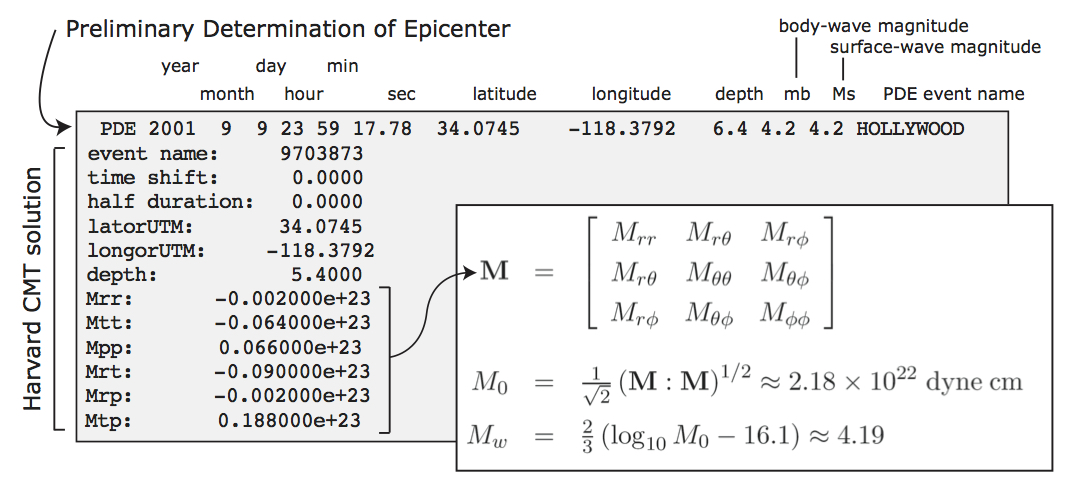
\includegraphics[width=0.8\textwidth]{figures/Hollywood_CMT.jpg}
\par
\end{centering}
\caption{\texttt{CMTSOLUTION} file based on the
format from the Harvard CMT catalog. \textbf{M} is the moment tensor,
$M_{0}${\small {} }is the seismic moment, and $M_{w}$ is the moment
magnitude.}
\label{fig:CMTSOLUTION-file}
\end{figure}
%
The \texttt{CMTSOLUTION} file should be edited in the following way:
\begin{itemize}
\item Set the latitude or UTM $x$ coordinate, longitude or UTM $y$ coordinate, depth of the source (in km).
\item Set the \texttt{time shift} parameter equal to $0.0$ (the solver
will not run otherwise.) The time shift parameter would simply apply
an overall time shift to the synthetics, something that can be done
in the post-processing (see Section \ref{sec:Process-data-and-syn}).
\item For point-source simulations (see finite sources, page \pageref{To-simulate-a})
we recommend setting the source half-duration parameter \texttt{half
duration} equal to zero, which corresponds to simulating a step source-time
function, i.e., a moment-rate function that is a delta function. If
\texttt{half duration} is not set to zero, the code will use a Gaussian
(i.e., a signal with a shape similar to a `smoothed triangle', as
explained in \citet{KoTr02a} and shown in Fig~\ref{fig:gauss.vs.triangle})
source-time function with half-width \texttt{half duration}. We prefer
to run the solver with \texttt{half duration} set to zero and convolve
the resulting synthetic seismograms in post-processing after the run,
because this way it is easy to use a variety of source-time functions
(see Section \ref{sec:Process-data-and-syn}). \citet{KoTr02a} determined
that the noise generated in the simulation by using a step source
time function may be safely filtered out afterward based upon a convolution
with the desired source time function and/or low-pass filtering. Use
the serial code \texttt{convolve\_source\_timefunction.f90} and the
script \texttt{convolve\_source\_timefunction.csh} for this purpose,
or alternatively use signal-processing software packages such as SAC
\urlwithparentheses{www.llnl.gov/sac}. Type
{\small
\begin{verbatim}
make xconvolve_source_timefunction
\end{verbatim}
}
to compile the code and then set the parameter \texttt{hdur} in \texttt{convolve\_source\_timefunction.csh}
to the desired half-duration.

\item The zero time of the simulation corresponds to the center of the triangle/Gaussian,
or the centroid time of the earthquake. The start time of the simulation
is $t=-1.5*\texttt{half duration}$ (the 1.5 is to make sure the moment
rate function is very close to zero when starting the simulation).
To convert to absolute time $t_{\mathrm{abs}}$, set
%
\begin{lyxcode}
$t_{\mathrm{abs}}=t_{\mathrm{pde}}+\texttt{time shift}+t_{\mathrm{synthetic}}$
\end{lyxcode}

where $t_{\mathrm{pde}}$ is the time given in the first line of the
\texttt{CMTSOLUTION}, \texttt{time shift} is the corresponding value
from the original \texttt{CMTSOLUTION} file and $t_{\mathrm{synthetic}}$
is the time in the first column of the output seismogram.
\end{itemize}
%
\begin{figure}[htp]
\begin{centering}
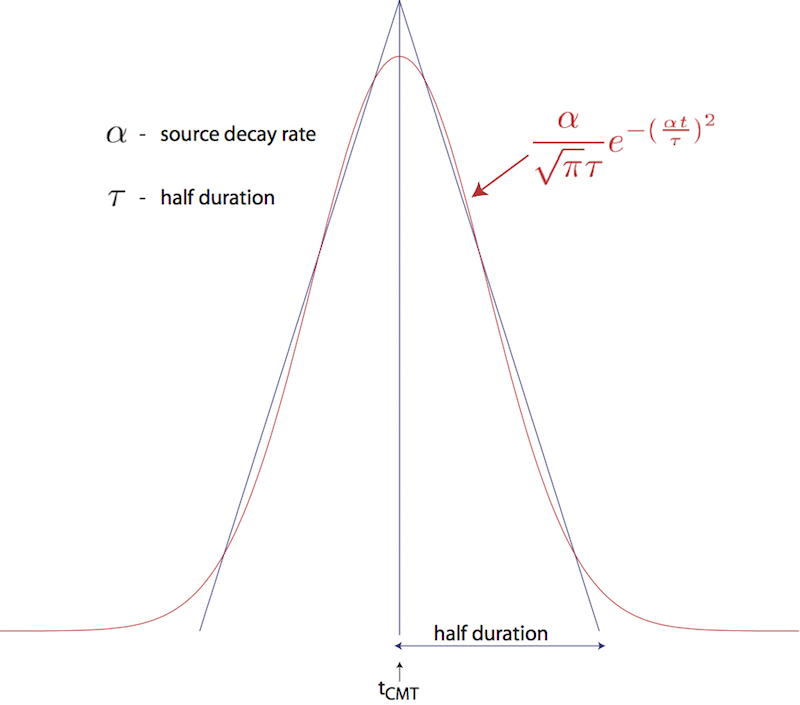
\includegraphics[width=3.5in]{figures/gauss_vs_triangle_mod.jpg}
\par
\end{centering}
\caption{Comparison of the shape of a triangle and the Gaussian function actually used.}
\label{fig:gauss.vs.triangle}
\end{figure}


If you know the earthquake source in strike/dip/rake format rather
than in \texttt{CMTSOLUTION} format, use the C code \texttt{SPECFEM3D\_GLOBE/utils/strike\_dip\_rake\_to\_CMTSOLUTION.c}
to convert it. The conversion formulas are given for instance in \citet{AkRi80}.
Note that the \citet{AkRi80} convention is slightly different from
the Harvard \texttt{CMTSOLUTION} convention (the sign of some components
is different). The C code outputs both.

Centroid latitude and longitude should be provided in geographical
coordinates. The code converts these coordinates to geocentric coordinates~\citep{DaTr98}.
Of course you may provide your own source representations by designing
your own \texttt{CMTSOLUTION} file. Just make sure that the resulting
file adheres to the Harvard CMT conventions (see Appendix~\ref{cha:Coordinates}).
Note that the first line in the \texttt{CMTSOLUTION} file is the Preliminary
Determination of Earthquakes (PDE) solution performed by the USGS
NEIC, which is used as a seed for the Harvard CMT inversion. The PDE
solution is based upon P waves and often gives the hypocenter of the
earthquake, i.e., the rupture initiation point, whereas the CMT solution
gives the `centroid location', which is the location with dominant
moment release. The PDE solution is not used by our software package
but must be present anyway in the first line of the file.

\label{To-simulate-a}To simulate a kinematic rupture, i.e., a finite-source
event, represented in terms of $N_{\mathrm{sources}}$ point sources,
provide a \texttt{CMTSOLUTION} file that has $N_{\mathrm{sources}}$
entries, one for each subevent (i.e., concatenate $N_{\mathrm{sources}}$
\texttt{CMTSOLUTION} files to a single \texttt{CMTSOLUTION} file).
At least one entry (not necessarily the first) must have a zero \texttt{time
shift}, and all the other entries must have non-negative \texttt{time
shift}. Each subevent can have its own half duration, latitude, longitude,
depth, and moment tensor (effectively, the local moment-density tensor).

Note that the zero in the synthetics does NOT represent the hypocentral
time or centroid time in general, but the timing of the \textit{center}
of the source triangle with zero \texttt{time shift} (Fig~\ref{fig:source_timing}).

Although it is convenient to think of each source as a triangle, in
the simulation they are actually Gaussians (as they have better frequency
characteristics). The relationship between the triangle and the gaussian
used is shown in Fig~\ref{fig:gauss.vs.triangle}. For finite fault
simulations it is usually not advisable to use a zero half duration
and convolve afterwards, since the half duration is generally fixed
by the finite fault model.

\vspace{1cm}


\noindent The \texttt{FORCESOLUTION} file should be edited in the
following way:
\begin{itemize}
\item Set the \texttt{time shift} parameter equal to $0.0$ (the solver
will not run otherwise.) The time shift parameter would simply apply
an overall time shift to the synthetics, something that can be done
in the post-processing (see Section \ref{sec:Process-data-and-syn}).
\item Set the \texttt{f0} parameter (the dominant frequency) of the Ricker source time
function when {\texttt{USE\_RICKER\_TIME\_FUNCTION}} is turned on
in the main parameter file {\texttt{Par\_file}}. In case that the
solver uses a (pseudo) Dirac delta source time function to represent
a force point source, a very short duration of five time steps is automatically set by default.
\item Set the latitude or UTM $x$ coordinate, longitude or UTM $y$ coordinate, depth of the source (in km).
\item Set the magnitude of the force source.
\item Set the components of a (non-unitary) direction vector for the force
source in the East/North/Vertical basis (see Appendix A for the orientation
of the reference frame).
\end{itemize}
\noindent Where necessary, set a \texttt{FORCESOLUTION} file in the
same way you configure a \texttt{CMTSOLUTION} file with $N_{\mathrm{sources}}$
entries, one for each subevent (i.e., concatenate $N_{\mathrm{sources}}$
\texttt{FORCESOLUTION} files to a single \texttt{FORCESOLUTION} file).
At least one entry (not necessarily the first) must have a zero \texttt{time
shift}, and all the other entries must have non-negative \texttt{time
shift}. Each subevent can have its own half latitude, longitude, depth,
\texttt{half duration} and force parameters.

\begin{figure}[H]
\begin{centering}
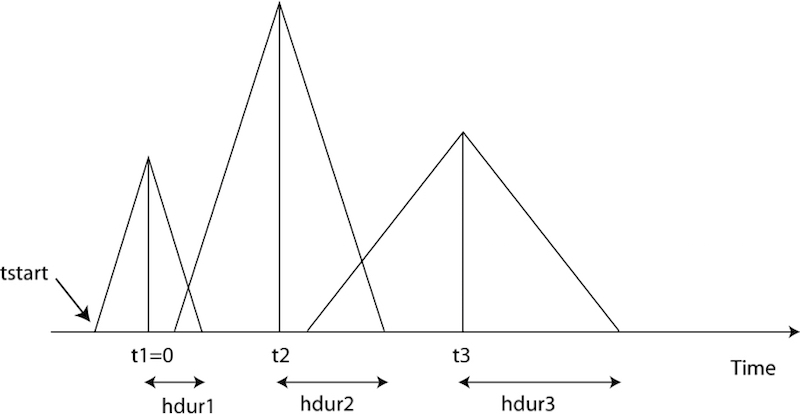
\includegraphics[width=4in]{figures/source_timing.jpg}
\par
\end{centering}
\caption{Example of timing for three sources. The center of the first source
triangle is defined to be time zero. Note that this is NOT in general
the hypocentral time, or the start time of the source (marked as tstart).
The parameter \texttt{time shift} in the \texttt{CMTSOLUTION} file
would be t1(=0), t2, t3 in this case, and the parameter \texttt{half
duration} would be hdur1, hdur2, hdur3 for the sources 1, 2, 3 respectively.}
{\small \label{fig:source_timing} }
\end{figure}

\vspace{1cm}

 In addition to inbuild source time function, the solver can also use an external source time function defined by the user. This option can be
activated by setting   \texttt{EXTERNAL\_SOURCE\_FILE} to true in \texttt{Par\_File} and by adding the name of the file
containing the source time function at the end of \texttt{FORCESOLUTION} or \texttt{CMTSOLUTION} files. The source time function file must
contain 2 columns with the current time and the amplitude of the soure function. The time step must be the same as used for the
simulation. Note  when the  \texttt{EXTERNAL\_SOURCE\_FILE} is set to false then the line with the external source time function file must not appear in
the files  \texttt{FORCESOLUTION} and \texttt{CMTSOLUTION} otherwise the solver will exit with an error.

\vspace{1cm}

The solver can calculate seismograms at any number of stations for
basically the same numerical cost, so the user is encouraged to include
as many stations as conceivably useful in the \texttt{STATIONS} file,
which looks like this:
%
\begin{figure}[H]
\begin{centering}
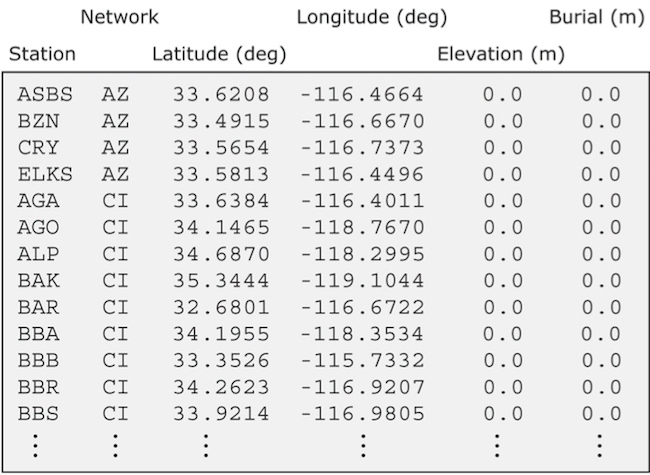
\includegraphics[width=4in]{figures/STATIONS_basin_explained.jpg}
\par
\end{centering}
\caption{Sample \texttt{STATIONS} file. Station latitude and longitude should
be provided in geographical coordinates. The width of the station
label should be no more than 32 characters (see \texttt{MAX\_LENGTH\_STATION\_NAME}
in the \texttt{constants.h} file), and the network label should be
no more than 8 characters (see \texttt{MAX\_LENGTH\_NETWORK\_NAME}
in the \texttt{constants.h} file).}
\label{fig:Sample-STATIONS-file.}
\end{figure}



Each line represents one station in the following format:
{\small
\begin{verbatim}
Station Network Latitude(degrees) Longitude(degrees) Elevation(m) burial(m)
\end{verbatim}
}
The solver \texttt{xspecfem3D} filters the list of stations in file
\texttt{DATA/STATIONS} to exclude stations that are not located within
the region given in the \texttt{Par\_file} (between \texttt{LATITUDE\_MIN}
and \texttt{LATITUDE\_MAX} and between \texttt{LONGITUDE\_MIN} and
\texttt{LONGITUDE\_MAX}). The filtered file is called \texttt{DATA/STATIONS\_FILTERED}.

Elevation and burial are generally applicable to geographical regions.
Burial is measured down from the top surface. For other problems in other
fields (ultrasonic testing, medical imaging etc...),
it may be confusing. We generally follow either of the following
procedures for those kind of problems:

Procedure 1:\\
============\\

- Always put the origin on the top of the model.\\

- Let's say you want to place two receivers at (x1,y1,z1) and
(x2,y2,z2). Your STATIONS file should look like:\\

BONE  GR  y1  x1  0.00  -z1\\
BONE  GR  y2  x2  0.00  -z2\\

Depending on the geometry of the models it may not work in some cases.\\

Procedure 2: (less recommended)\\
============\\

- Open setup/constants.h.in file and change the line
logical, parameter :: USE\_SOURCES\_RECEIVERS\_Z = .false.\\
\\
to\\
\\
logical, parameter :: USE\_SOURCES\_RECEIVERS\_Z = .true.\\
\\
configure the package and compile.\\

- Let's say you want to place two receivers at (x1,y1,z1) and
(x2,y2,z2). Your STATIONS file should look like:\\
\\
BONE  GR  y1  x1  0.00  z1\\
BONE  GR  y2  x2  0.00  z2\\
\\
The option set to .true. in 1 will discard the elevation and set
burial as the $z$ coordinate.\\
\\
Third column is Y and Fourth is X due to the latitude/longitude convention.\\
\\
You can replace the station name "BONE" with any word of length less
than 32, and the network name "GR" with any word of length less than
8.\\
\\
You can always plot OUTPUT\_FILES/sr.vtk file in ParaView to check the
source/receiver locations after your simulation.\\

Solver output is provided in the \texttt{OUTPUT\_FILES} directory
in the \texttt{output\_solver.txt} file. Output can be directed to
the screen instead by uncommenting a line in \texttt{constants.h}:
\begin{verbatim}
! uncomment this to write messages to the screen
! integer, parameter :: IMAIN = ISTANDARD_OUTPUT
\end{verbatim}
On PC clusters the seismogram files are generally written to the local
disks (the path \texttt{LOCAL\_PATH} in the \texttt{Par\_file}) and
need to be gathered at the end of the simulation.

While the solver is running, its progress may be tracked by monitoring
the `\texttt{\small timestamp{*}}' files in the \texttt{\small OUTPUT\_FILES/} directory. These tiny
files look something like this:
{\small
\begin{verbatim}
Time step #          10000
Time:     108.4890      seconds
Elapsed time in seconds =    1153.28696703911
Elapsed time in hh:mm:ss =     0 h 19 m 13 s
Mean elapsed time per time step in seconds =     0.115328696703911
Max norm displacement vector U in all slices (m) =     1.0789589E-02
\end{verbatim}
}
The \texttt{\small timestamp{*}} files provide the
\texttt{\small Mean elapsed time per time step in seconds}, which may be used
to assess performance on various machines (assuming you are the only
user on a node), as well as the
\texttt{\small Max norm displacement vector U in all slices~(m)}.
If something is wrong with the
model, the mesh, or the source, you will see the code become unstable
through exponentially growing values of the displacement and fluid
potential with time, and ultimately the run will be terminated by
the program. You can control the rate at which the timestamp files
are written based upon the parameter
\texttt{\small NTSTEP\_BETWEEN\_OUTPUT\_INFO}
in the \texttt{\small Par\_file}.

Having set the \texttt{Par\_file} parameters, and having provided
the \texttt{CMTSOLUTION} (or the \texttt{FORCESOLUTION}) and \texttt{STATIONS}
files, you are now ready to launch the solver! This is most easily
accomplished based upon the \texttt{go\_solver} script (See Chapter
\ref{cha:Scheduler} for information about running through a scheduler,
e.g., LSF). You may need to edit the last command at the end of the
script that invokes the \texttt{mpirun} command. The \texttt{runall}
script compiles and runs both \texttt{xgenerate\_databases} and \texttt{xspecfem3D}
in sequence. This is a safe approach that ensures using the correct
combination of distributed database output and solver input.

It is important to realize that the CPU and memory requirements of
the solver are closely tied to choices about attenuation (\texttt{ATTENUATION})
and the nature of the model (i.e., isotropic models are cheaper than
anisotropic models). We encourage you to run a variety of simulations
with various flags turned on or off to develop a sense for what is
involved.

For the same model, one can rerun the solver for different events
by simply changing the \texttt{CMTSOLUTION} or \texttt{FORCESOLUTION}
file, or for different stations by changing the \texttt{STATIONS}
file. There is no need to rerun the \texttt{xgenerate\_databases}
executable. Of course it is best to include as many stations as possible,
since this does not add to the cost of the simulation.

We have also added the ability to run several calculations (several earthquakes)
in an embarrassingly-parallel fashion from within the same run;
this can be useful when using a very large supercomputer to compute
many earthquakes in a catalog, in which case it can be better from
a batch job submission point of view to start fewer and much larger jobs,
each of them computing several earthquakes in parallel.
To turn that option on, set parameter \texttt{NUMBER\_OF\_SIMULTANEOUS\_RUNS}
to a value greater than 1 in file setup/constants.h.in before
configuring and compiling the code.
When that option is on, of course the number of processor cores used to start
the code in the batch system must be a multiple of \texttt{NUMBER\_OF\_SIMULTANEOUS\_RUNS},
all the individual runs must use the same number of processor cores,
which as usual is \texttt{NPROC} in the input file \texttt{DATA/Par\_file},
and thus the total number of processor cores to request from the batch system
should be \texttt{NUMBER\_OF\_SIMULTANEOUS\_RUNS $\times$ NPROC}.
All the runs to perform must be placed in directories called \texttt{run0001}, \texttt{run0002}, \texttt{run0003} and so on (with exactly four digits)
and you must create a link from the root directory of the code
to the first copy of the executable programs by typing \texttt{ln -s run0001/bin bin}.


\section{Note on the viscoelastic model used}

\noindent
The model used is a constant $Q$, thus with no dependence on frequency ($Q(f)$ = constant).
See e.g. \cite{BlKoChLoXi16}. \\

\noindent
However in practice for technical reasons it is approximated based on the sum of different Generalized Zener body mechanisms
and thus the code outputs the band in which the approximation is very good, outside of that range it can be less accurate.
The logarithmic center of that frequency band is the \texttt{ATTENUATION\_f0} parameter defined (in Hz) in input file \texttt{DATA/Par\_file}.

